\documentclass{report}
\usepackage{graphicx}
\usepackage{booktabs}
\usepackage{amsmath,amssymb}
\renewcommand{\thesection}{\arabic{section}}

\author{Trinh Thanh Vinh}
\title{Labwork 5: Gaussian Blur Convolution}

\begin{document}
\maketitle

\section{Objective}
The goal of this labwork is to compare an image blur program on a CPU and a CUDA GPU. Three versions were tested: CPU, GPU with shared memory, and GPU without shared memory.

\section{Method}
The input image size was $6000 \times 2962$, or 17,772,000 pixels. The GPU versions were tested with three block sizes: $8 \times 8$, $16 \times 16$, and $32 \times 32$. The measured execution times were then compared.

\section{Results}
\begin{table}[h]
\centering
\begin{tabular}{lcc}
\hline
Implementation & Block size & Time (s) \\
\hline
CPU & N/A & 187.7 \\
GPU with shared memory & $8 \times 8$ & 0.064995 \\
GPU with shared memory & $16 \times 16$ & 0.061779 \\
GPU with shared memory & $32 \times 32$ & 0.066184 \\
GPU without shared memory & $8 \times 8$ & 0.063658 \\
GPU without shared memory & $16 \times 16$ & 0.061930 \\
GPU without shared memory & $32 \times 32$ & 0.061409 \\
\hline
\end{tabular}
\caption{Execution time of the two GPU versions.}
\end{table}

\begin{figure}[h]
\centering
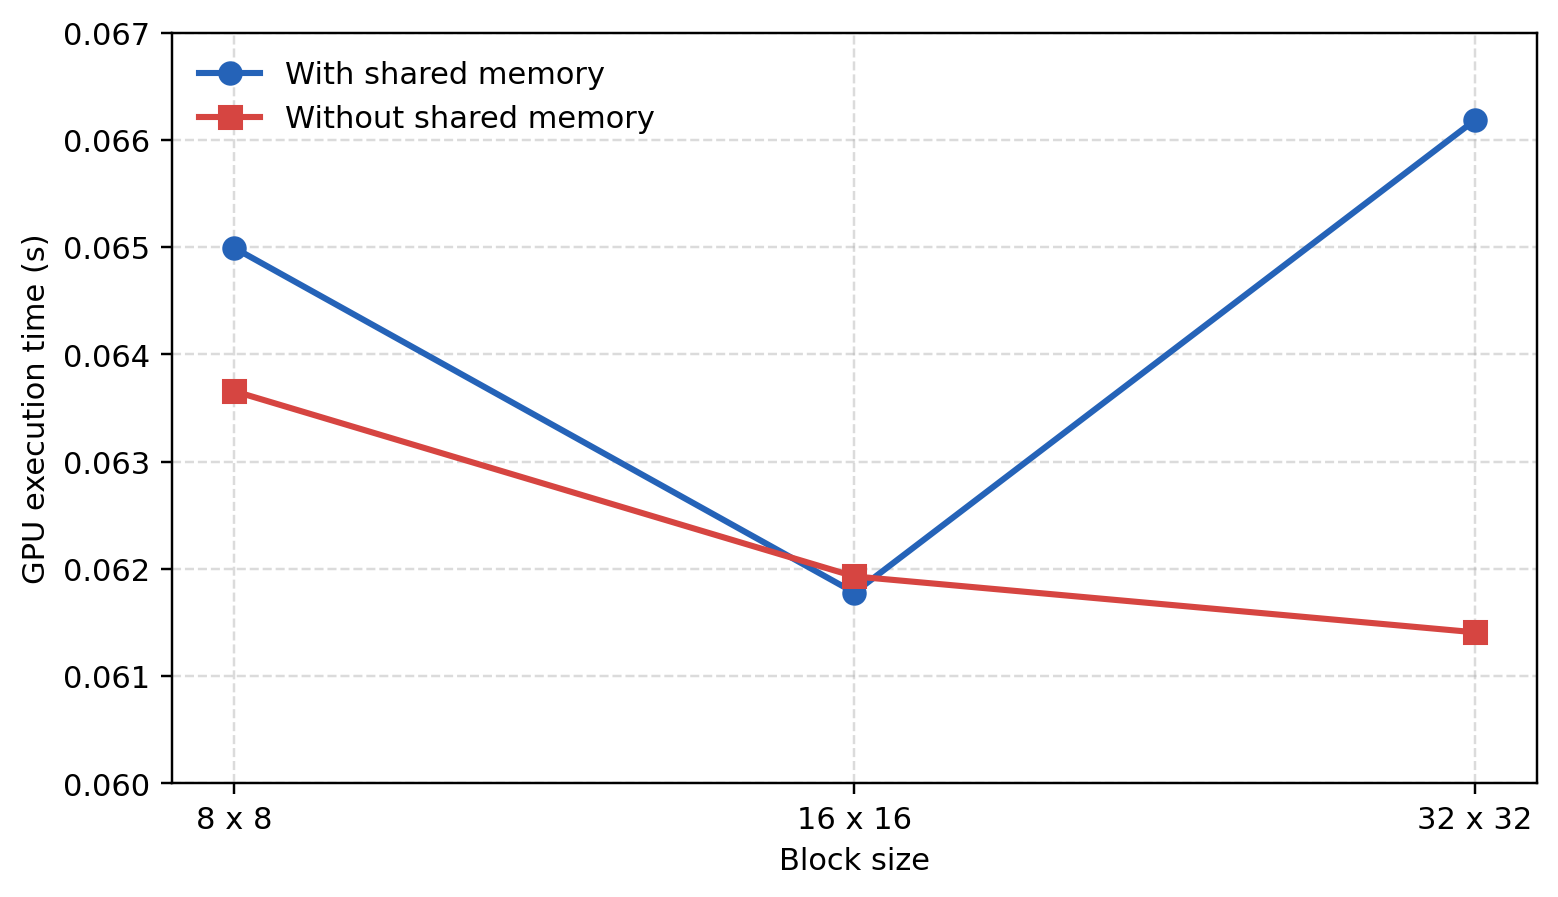
\includegraphics[width=0.78\textwidth]{gpu_block_time.png}
\caption{Block size versus execution time for the two GPU versions.}
\end{figure}

The fastest shared-memory result was 0.061779 seconds with a $16 \times 16$ block. The fastest result overall was 0.061409 seconds without shared memory, using a $32 \times 32$ block.

\section{Discussion}
Changing block size did not significantly change the GPU time. With shared memory, the $16 \times 16$ block was the best choice. Without shared memory, performance improved as the block size increased. In this test, shared memory did not give a clear benefit.
\end{document}